\documentclass{article}

\usepackage{graphicx}
\usepackage{tikz}
\usepackage{tikzsymbols}
\usetikzlibrary{calc,patterns,shapes.geometric}
\pagestyle{empty}
\usepackage[margin=0pt]{geometry}
\geometry{papersize={14in,12in}}

\def\centerarc[#1](#2)(#3:#4:#5){\draw[#1] ($(#2)+({#5*cos(#3)},{#5*sin(#3)})$) arc (#3:#4:#5);}

\begin{document}
	\begin{figure}
		\centering
		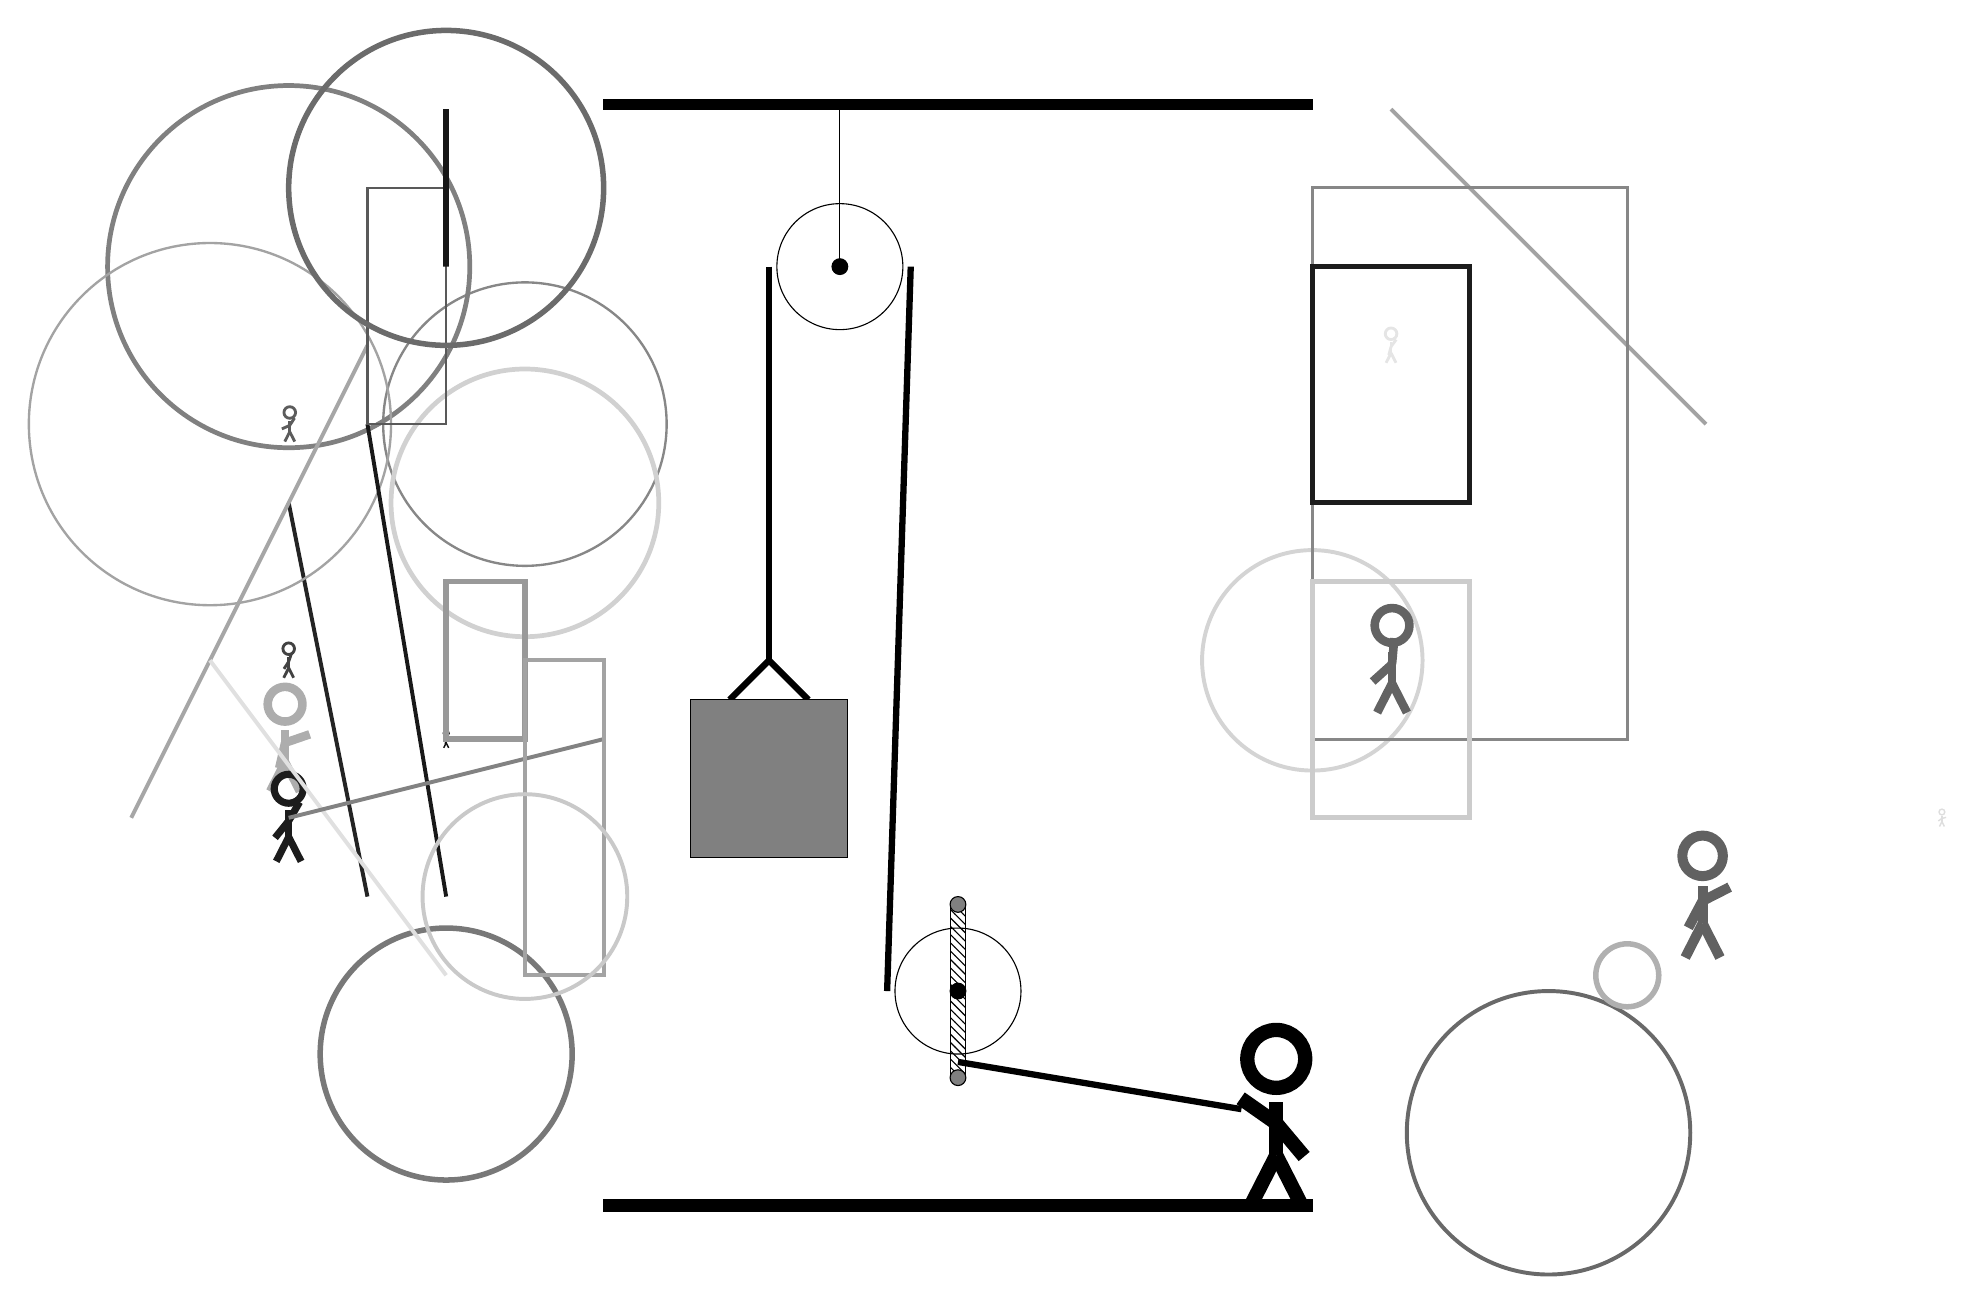
\begin{tikzpicture}
			%%%%% START %%%%%
			
			\draw[fill=black] (-2, 14) rectangle (7, 14.125);
			
			\draw [line width=0.4mm, color=black!56](14, 7) circle (0.0);
			
			\draw[line width=0.5mm, color=black!36](8, 14) -- (12, 10);
			\node[line width=0.2mm, color=black!32] at (-6, 6) {\Strichmaxerl[6][77][19]};
			\node[line width=0.3mm, color=black!10] at (8, 11) {\Strichmaxerl[2][75][54]};
			\draw [line width=0.5mm, color=black!59](10, 1) circle (1.8);
			
			\draw [line width=0.3mm, color=black!47](-3, 10) circle (1.8);
			\node[line width=0.3mm, color=black!13] at (15, 5) {\Strichmaxerl[1][35][15]};
			
			\draw[line width=0.5mm, color=black!86](-6, 9) -- (-5, 4);
			\draw [line width=0.7mm, color=black!53](-4, 2) circle (1.6);
			
			\node[line width=0.5mm, color=black!74] at (-6, 7) {\Strichmaxerl[2][57][71]};
			\draw [line width=0.6mm, color=black!50](-6, 12) circle (2.3);
			
			\node[line width=0.5mm, color=black!64] at (-6, 10) {\Strichmaxerl[2][24][57]};
			\node[line width=0.3mm, color=black!62] at (12, 4) {\Strichmaxerl[7][62][27]};
			
			\draw [line width=0.7mm, color=black!31](11, 3) circle (0.4);
			\node[line width=0.6mm, color=black!89] at (-6, 5) {\Strichmaxerl[5][51][60]};
			\draw [line width=0.5mm, color=black!17](7, 7) circle (1.4);
			
			\node[line width=0.7mm, color=black!93] at (-4, 6) {\Strichmaxerl[1][78][54]};
			
			\draw [line width=0.3mm, color=black!36](-7, 10) circle (2.3);
			\draw [line width=0.6mm, color=black!18](-3, 9) circle (1.7);
			\draw[line width=0.5mm, color=black!35](-5, 11) -- (-8, 5);
			\draw[line width=0.5mm, color=black!12](-4, 3) -- (-7, 7);
			
			\draw[line width=0.5mm, color=black!90](-4, 4) -- (-5, 10);
			\draw[line width=0.5mm, color=black!49](-2, 6) -- (-6, 5);
			\draw[line width=0.4mm, color=black!47] (7, 6) rectangle (11, 13);
			\draw[line width=0.3mm, color=black!65] (-4, 13) rectangle (-5, 10);
			\draw[line width=0.6mm, color=black!89] (9, 12) rectangle (7, 9);
			\draw [line width=0.7mm, color=black!58](-4, 13) circle (2.0);
			\draw[line width=0.7mm, color=black!40] (-3, 6) rectangle (-4, 8);
			
			\draw[line width=0.5mm, color=black!36] (-2, 3) rectangle (-3, 7);
			
			\draw[line width=0.6mm, color=black!20] (7, 8) rectangle (9, 5);
			\draw[line width=0.7mm, color=black!91] (-4, 12) rectangle (-4, 14);
			
			\draw [line width=0.5mm, color=black!21](-3, 4) circle (1.3);
			\node[line width=0.5mm, color=black!61] at (8, 7) {\Strichmaxerl[6][42][85]};
			
			
			\draw (1, 12) circle (0.8);
			\draw[fill=black] (1, 12) circle (0.1);
			\draw (1, 14) -- (1, 12);
			
			\draw[fill=white](2.5, 2.8) circle (0.8);
			\draw[fill=black] (2.5, 2.8) circle (0.1);
			\draw[pattern=north west lines, pattern color=black] (2.4, 3.9) rectangle (2.6, 1.7);
			\draw[fill=black!50] (2.5, 3.9) circle (0.1);
			\draw[fill=black!50] (2.5, 1.7) circle (0.1);
			
			\draw[line width=0.8mm] (-0.4, 6.5) -- (0.1, 7.0) -- (0.6, 6.5);
			\draw[fill=black!50] (-0.9, 6.5) rectangle (1.1, 4.5);
			
			\draw[line width=0.8mm] (0.1, 12) -- (0.1, 7.0);
			\centerarc[line width=0.8mm](1, 12)(0:180:0.9);
			\draw[line width=0.8mm](1.9, 12) -- (1.6, 2.8);
			\centerarc[line width=0.8mm](2.5, 2.8)(180:270:0.9);
			\draw[line width=0.8mm](2.5, 1.9) -- (6.1, 1.3);
			
			\node at (6.5, 1.2) {\Strichmaxerl[10][-35][-50]};
			
			\draw[fill=black] (-2, 0) rectangle (7, 0.15);
			
			%%%%% END %%%%%
		\end{tikzpicture}
	\end{figure}	
\end{document}